Los archivos APK, que son archivos instalables en Android que viene de la sigla Application Package es una variante de los ficheros JAR, de Java Archive, que es un paquete que contiene los archivos necesarios para instalar o hacer correr una aplicación Java.
\\\\
A su vez, un JAR es comparable a un ZIP pero la mayoría de las veces viene sin compresión.
\\\\
    Además, Java, el lenguaje de programación de las aplicaciones Android, es un lenguaje que se compila a bytecode, que es un intermediario entre código de máquina y binario. Este bytecode se hace correr sobre una máquina virtual Java.
\\\\
Finalmente, esto quiere decir que Java es precompilado o preparado para correr más rápido sobre una máquina virtual de Java y gracias a esto es posible lograr programas multiplataforma. Basta con generar una máquina virtual para otro sistema y el programa ya debería correr.
\\\\
El problema de esto es que la capacidad de poder realizar ingeniería inversa es mayor, como el código es intermedio, es más cercano a lo que se programó originalmente.
\\\\
El software APK Studio permite realizar esta ingeniería inversa y generar el árbol de directorios y los instructivos de Java en Smali. Smali es otra forma de decir Assembly (Assembler)
    
        \begin{figure}[H]
  \begin{center}
    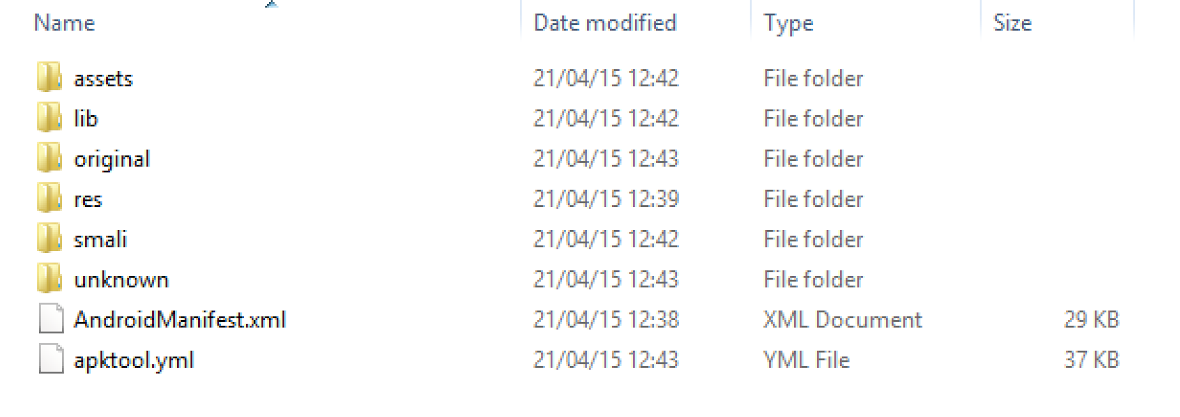
\includegraphics[width=0.9\textwidth]{imagenes/fig26.png}
    \caption{Decompilación del APK Studio}
  \end{center}
\end{figure}
    
En la figura 3 podemos ver la descompilación que realizó APK Studio. En Assets y RES se encuentran las imágenes de la aplicación, en Original encontramos los manifiests (archivos de configuración de muestra de la aplicación en android).
\\\\
Dentro de Smali/com/waze encontramos los assembly de los diferentes trozos de código.
\\\\
Como queremos un código más entendible, transformamos Smali a Java con smali2java ([7]).


    \begin{figure}[H]
  \begin{center}
    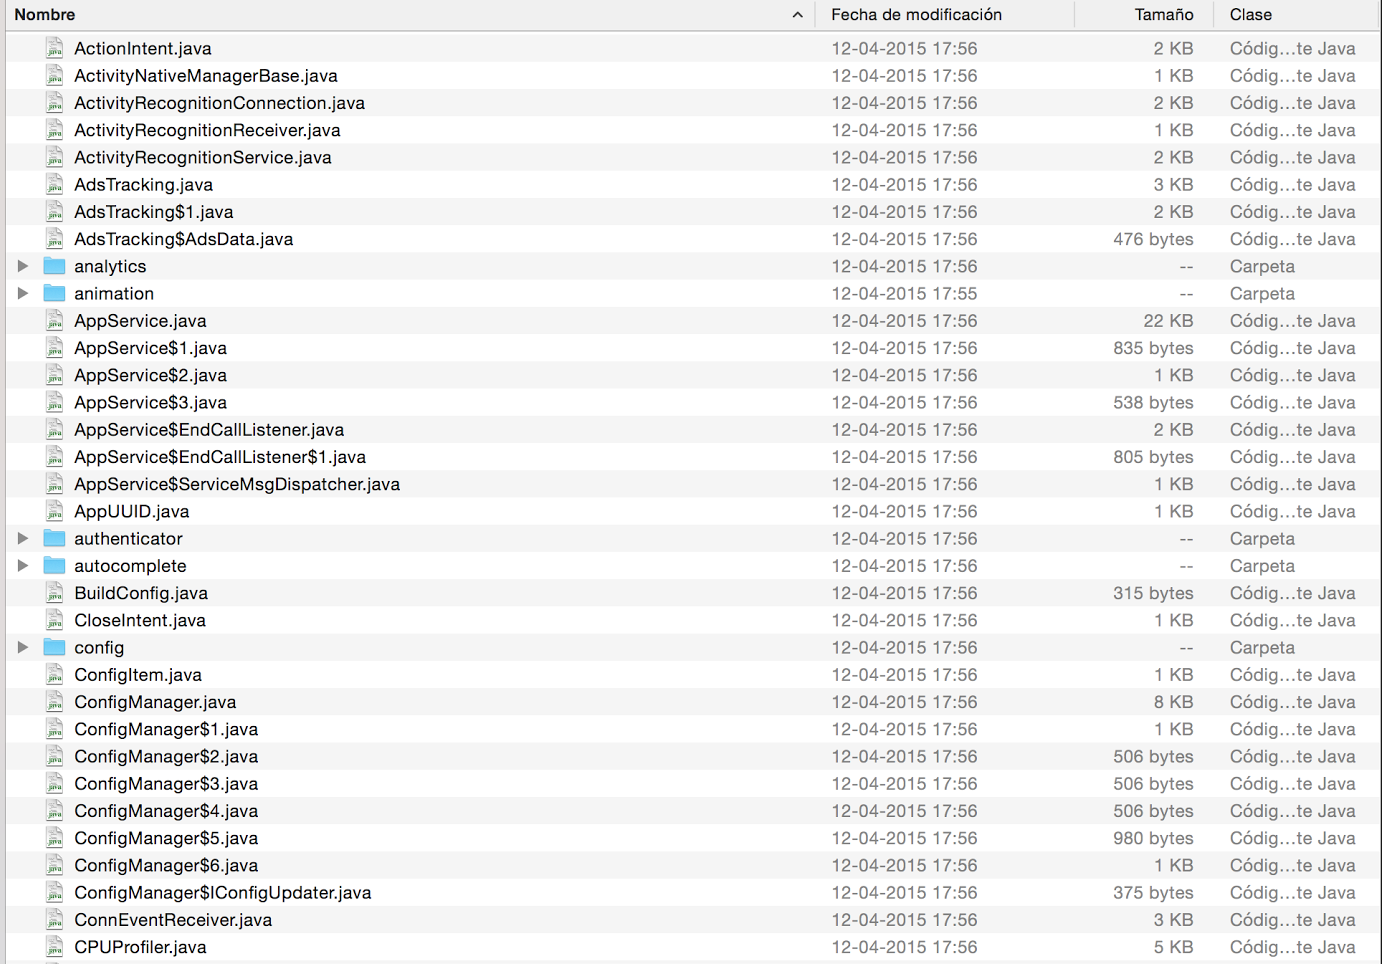
\includegraphics[width=0.9\textwidth]{imagenes/fig27.png}
    \caption{Archivos Smali convertidos a Java}
  \end{center}
\end{figure}

En la figura 4 ya tenemos el código convertido en Java. Aprovechando esto, primero buscamos alguna referencia de alguna base de datos:

    \begin{figure}[H]
  \begin{center}
    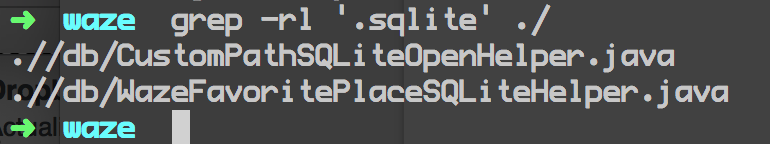
\includegraphics[width=0.8\textwidth]{imagenes/fig28.png}
    \caption{Busqueda de referencia de una base de datos}
  \end{center}
\end{figure}

En el primer archivo (Figura 5) solo hay configuración de la aplicación para utilizar una ruta específica para el fichero SQLite y en el segundo, encontramos una sentencia SQL:

    \begin{figure}[H]
  \begin{center}
    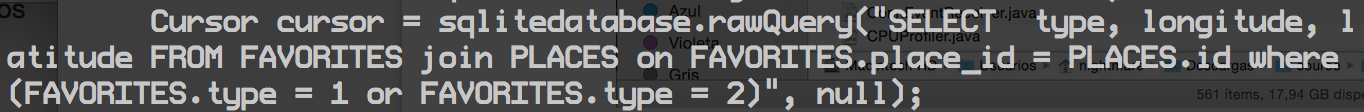
\includegraphics[width=0.8\textwidth]{imagenes/fig29.png}
    \caption{Sentencia sql}
  \end{center}
\end{figure}

En la figura 26 podemos ver que las ubicaciones favoritas (función de Waze) se guarda en el archivo SQLite.
\\\\
Comenzamos la búsqueda de direcciones pero notamos que las direcciones comienzan con “waze://”, esto en una aplicación quiere decir que se definió un esquema único para la aplicación (Esto es, que desde cualquier otra aplicación o navegador, se puede ejecutar Waze mediante una URL ( [9]).

    \begin{figure}[H]
  \begin{center}
    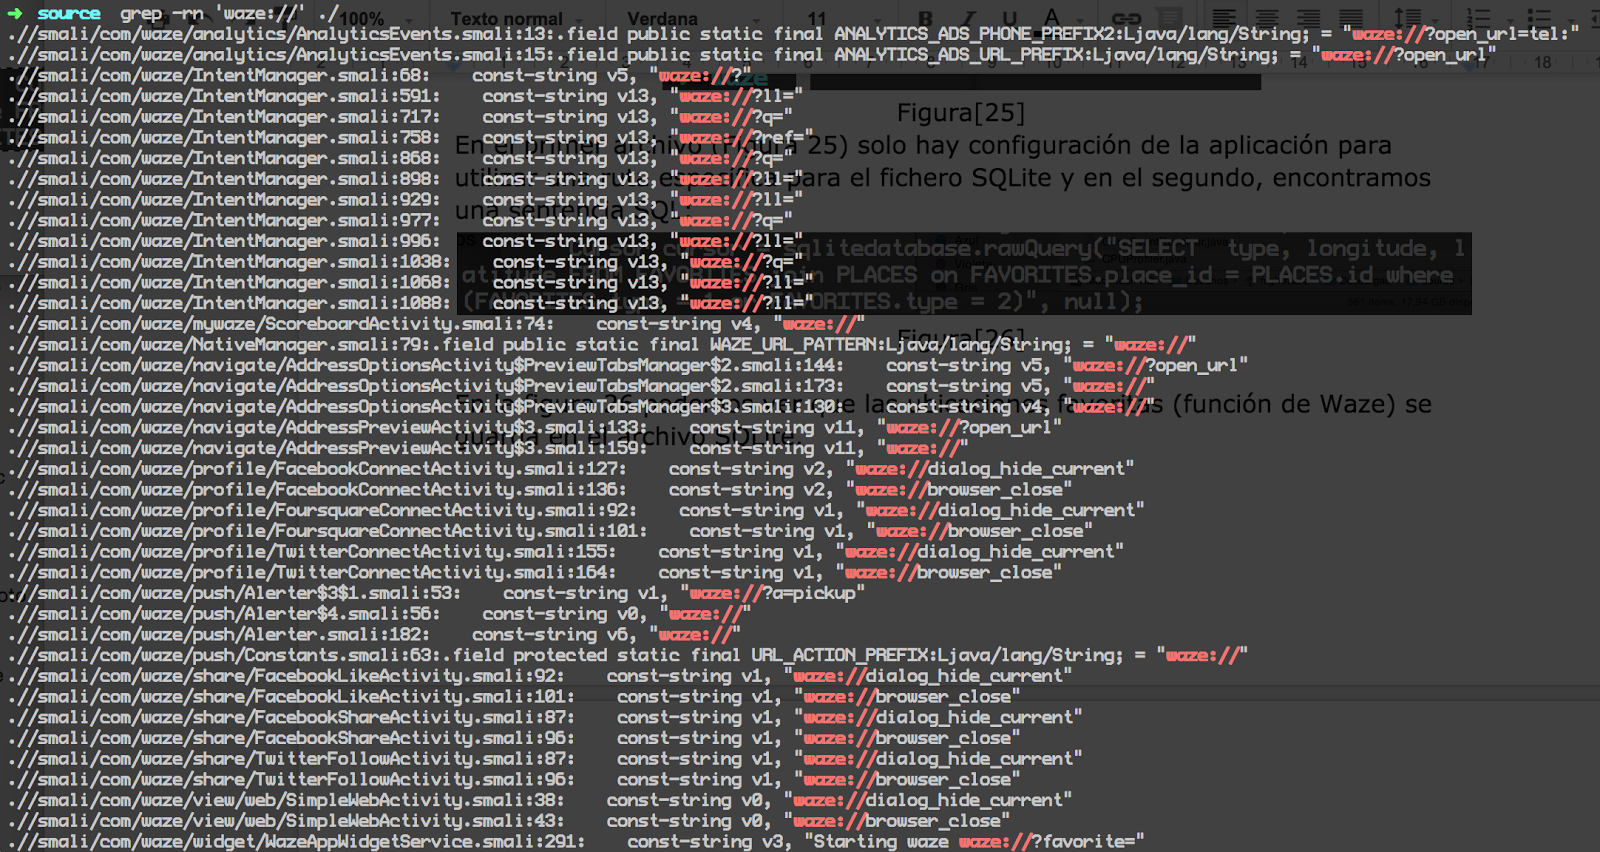
\includegraphics[width=0.9\textwidth]{imagenes/fig30.png}
    \caption{Busqueda de direcciones que comienzan con “waze://”}
  \end{center}
\end{figure}

Investigando, las aplicaciones deben realizar una instanciación de la clase Intent para modificar el comportamiento con una URL específica de una aplicación.
\\\\
Los ficheros de IntentManager encontramos lo siguiente:

    \begin{figure}[H]
  \begin{center}
    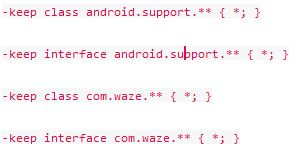
\includegraphics[width=0.8\textwidth]{imagenes/contFig30.JPG}
    \caption{Cotenido de los ficheros de IntentManager}
  \end{center}
\end{figure}


Lo que quiere decir que utilizaron técnicas de ofuscación de código para ocultar la URL original.
\\\\
La ofuscación de código se utiliza para justamente ocultar partes del código sensibles, forzando a que sean compiladas en el momento de crear el APK.
\\\\
En toda solicitud URL hay ofuscación de código. ([8]).